\documentclass{article}
\usepackage[top=1.0in,bottom=1.0in,left=1.0in,right=1.0in]{geometry}
\usepackage{amsmath,amssymb,amsthm,amsfonts}
\usepackage[utf8]{inputenc}
\usepackage[T2A]{fontenc}
\usepackage[english,russian]{babel}
\usepackage{hyperref}
\usepackage{graphicx}

\title{Triptych: логарифмически масштабируемые связываемые кольцевые подписи и их применение}
\author{Саранг Ноезер (Sarang Noether) и Брендон Гуделл (Brandon Goodell) \\ Исследовательская лаборатория Monero (Monero Research Lab) \\ \texttt{\{sarang,surae\}.noether@protonmail.com}}
\date{24 января, 2020}

\newcommand{\G}{\mathbb{G}}
\newcommand{\F}{\mathbb{F}}
\newcommand{\com}{\operatorname{Com}}
\newcommand{\hs}{\mathcal{H}}
\newcommand{\hp}{\mathbb{H}}

\newcommand{\A}{\mathcal{A}}

\newcommand{\sumi}{\sum_{i=0}^{n-1}}
\newcommand{\sumj}{\sum_{j=0}^{m-1}}
\newcommand{\sumk}{\sum_{k=0}^{N-1}}

\newtheorem{theorem}{Теорема}
\theoremstyle{definition}
\newtheorem{definition}{Определение}

\begin{document}

\maketitle


\begin{abstract}
Кольцевые подписи являются распространённой структурой, используемой с целью сокрытия реального подписанта среди неинтерактивного набора публичных ключей, указываемых во время подписания. В отличие от предшествующих подходов, предполагавших линейность размера подписи в рамках группы анонимных подписантов, существующие оптимальные решения требуют либо использования централизованных доверенных настроек, либо создания логарифмически масштабируемых подписей. Тем не менее некоторые подходы также обеспечивают связываемость, свойство, используемое для определения того, подписывал ли ранее подписант какое-либо другое сообщение, возможно, с ограничениями по выбору членов анонимной группы. Нами предлагается Triptych, семейство не требующих доверенных настроек связываемых кольцевых подписей, в основе которых лежат обобщённые доказательства с нулевым разглашением по открытым обязательствам до нуля. Нами приводятся примеры применения Triptych в составе протоколов транзакций с сокрытием подписанта путём расширения схемы до открытых параллельных обязательств в независимых анонимных группах. Подписи являются логарифмически масштабируемыми в рамках размера анонимной группы, и, несмотря на то, что сложность верификации линейна, доказательства допускают возможность групповой верификации. Мы демонстрируем, что в случае с практичным с точки зрения использования размером анонимной группы в составе распределённых протоколов Triptych обеспечивает конкурентные показатели даже при простом варианте реализации.
\end{abstract}


\section{Введение}
Будучи впервые представленными в работе \cite{rivest} wв связи с группами RSA, кольцевые подписи позволили подписывать сообщения при помощи не определяемого предварительно набора публичных ключей без привлечения доверенного менеджера группы. Предшествующим конструкциям не хватало гибкости, и требовались либо централизованные настройки ключей, либо наличие фиксированных групп подписантов. В более поздней работе \cite{bender} были предложены более устойчивые модели безопасности, обеспечивающие невозможность фальсификации и анонимность и учитывающие реальные модели угроз, когда у злоумышленника имеется возможность взломать ключи, убедить честных подписантов включить эти ключи в анонимную группу или же заполучить подписи заранее.

Так как кольцевая подпись включает в себя анонимную группу публичных ключей, один из которых принадлежит настоящему подписанту, обнаружение того факта, что для подписания использовался тот же ключ, требуется дополнительное свойство, называемой связываемостью. Связываемая кольцевая подпись \cite{lsag} позволяет верификаторам определить, подписывал ли (неизвестный) подписант сообщения и другие сообщения. Такая схема может использоваться в процессе выборов, когда необходимо гарантировать анонимность голосования, но при этом свой голос можно было отдать лишь единожды по определённому вопросу. Схема, предложенная в работе \cite{lsag}, имеющая ту же секретную структуру хеша, что и схема, приведённая в работе \cite{schnorr}, представляет собой определённый интерес благодаря потенциальной гибкости с точки зрения связывания; несмотря на то, что в этом случае возможность связывания ограничена группами выбираемых, но неизменяемых анонимных подписантов, она позволяет осуществлять связывание на основе конкретного случая. В ещё одной недавно появившейся работе \cite{backes} описано свойство связываемой анонимности, предполагающее использование наборов подписей и ограничение возможного умышленного повреждения ключей. Другие связанные с этим интересные свойства, такие как отслеживаемость \cite{fs,f}, подразумевают более сильные возможности, когда попытка подписать два сообщения при помощи одного и того же ключа позволяет верификатору идентифицировать подписанта.

Связываемые кольцевые подписи уже нашли своё применение в некоторых протоколах транзакций с сокрытием подписанта. В этом случае транзакции подтверждаются кольцевой подписью, в которой группа анонимных подписантов состоит из ранее сгенерированных выходов транзакций. Подпись демонстрирует, что подписант обладает приватным ключом к одному из таких выходов, но кто именно является подписантом не раскрывается, а свойство связываемости используется для того, чтобы убедить верификаторов в том, что выход не был использован ранее в другой подписи (что означало бы попытку двойной траты).

Практическим вопросом, в случае с применением связываемых кольцевых подписей в рамках протокола транзакций, является масштабирование размера подписи и времени верификации относительно размера анонимной группы. В случае с распространёнными схемами, подобными тем, что описаны в работах \cite{mlsag,clsag}, размер подписи и время верификации масштабируются линейно относительно размера анонимной группы, скрывающей подписанта; так как подобные подписи, как правило, включаются в публичную распределённую структуру данных, такую как блокчейн, существует баланс между размером анонимной группы и требованиями к хранению и верификации. Недавняя доработка протокола позволяет избежать ограничений, связанных с размером. Например, в работе \cite{rct3} авторами предлагается протокол конфиденциальных транзакций, основанный на системе доказательства, размер которой масштабируется логарифмически относительно размера анонимной группы, и включающий в себя способ демонстрации баланса; доказательство диапазона обязательства по сумме облегчается в других схемах, подобных представленной в работе \cite{bulletproofs}.
В работе \cite{omniring} авторами используется более общий метод доказательства, пригодный для достижения той же цели. Тем не менее протокол демонстрирует улучшения с точки зрения сокращения размера за счёт интеграции доказательств диапазона обязательства напрямую в схему доказательства благодаря логарифмически масштабируемому размеру доказательства.

Другие протоколы транзакций с сокрытием подписанта, в основе которых не лежат связываемые кольцевые подписи, демонстрируют более конкурентные показатели производительности. Например, протоколы, подобные описанному в работе \cite{zcash}, обеспечивают теоретически максимальное сокрытие подписанта за счёт применения, помимо прочих, доказательства Меркла с нулевым разглашением, имеющее крайне малый размер и незначительное время верификации, но это достигается за счёт использования доверенных структурированных настроек, являющихся неизменным атрибутом, лежащим в основе системы доказательства \cite{groth16}.
Как и в этой работе, протокол транзакций, описанный в работе \cite{lelantus}, также основан на том, что предлагается в работе \cite{groth}. Тем не менее он работает с обязательствами, схожими с теми, что используются в работе \cite{zerocoin}, например, но также указывает суммы и имеет ограничения по адресации и отслеживанию отправителя.


\subsection{Наш вклад}
Нами предлагается семейство связываемых кольцевых подписей под названием Triptych. Наши схемы представляют собой связываемую генерализацию системы доказательства одного из многих обязательств по нулю Грота \cite{groth} с оптимизацией Бутля \cite{bootle}, использованной для улучшения масштабирования размера доказательства и сложности верификации. В случае реализации самой простой версии Triptych доказывающая сторона демонстрирует, что ей известно открытие обязательства по нулю в рамках набора обязательств, а также, что ею при помощи того же открытия был построен связующий тег, в результате чего была получена связываемая кольцевая подпись. Затем мы изменяем определения кольцевой подписи Грота, включая в них свойство связываемости и ещё одно связываемое с ней свойство невозможности выборки.

В расширение Triptych нами включается множество независимых наборов обязательств. В этом случае доказывающая сторона делает то же, что и ранее, чтобы продемонстрировать, что ей известно открытие обязательства в одном наборе, равно как и структура связующего тега. Тем не менее доказательство также демонстрирует, что доказывающей стороне известно открытие обязательства в том же самом месте во всех других наборах. Такая схема имеет непосредственное применение; в случае с некоторыми протоколами транзакций с сокрытием подписанта входы транзакций являются обязательствами по нулю, в отношении которых подписантом демонстрируется знание открытия. Каждое обязательство сопровождается ещё одним обязательством по сумме входа; гомоморфно смещая эти обязательства, и за счёт тщательного выбора случайности обязательства доказывающая сторона может продемонстрировать сбалансированность определённой транзакции.

Мы показываем, что Triptych позволяет создавать подписи, обладающие конкурентными показателями производительности в сравнении с другими современными связываемыми кольцевыми подписями, используемыми в случае с ограниченными по размеру анонимными группами. Нами подчёркивается, что подобные схемы также требуют линейного времени верификации, а это означает, что размер анонимной группы, используемый на практике, вероятно, будет ограничен по причинам производительности.


\section{Предварительная информация}
\subsection{Публичные параметры}
Допустим, \begin{math}\mathbb{G}\end{math} является циклической группой, в рамках которой задача логарифмирования является сложной, и допустим, что $\F$ является полем скалярных величин \begin{math}\mathbb{G}\end{math}.
Допустим $\hs: \{0,1\}^* \to \F$ является криптографической хеш-функцией. Допустим, $G$ и $H$ являются генераторами \begin{math}\mathbb{G}\end{math} с неизвестным отношением по дискретному логарифму.
Допустим, $N = n^m$ является параметром размера, где $n > 1$ и $m > 1$.
Допустим, $\{G_{j,i}\}_{j,i=0}^{m-1,n-1}$ является набором генераторов \begin{math}\mathbb{G}\end{math} с неизвестным отношением друг к другу по дискретному логарифму, к $G$ и $H$.
Допустим, $U$ является генератором \begin{math}\mathbb{G}\end{math}.
Следует отметить, что все генераторы могут быть созданы с публичной случайностью; например, здесь вполне подойдёт соответствующая хеш-функция с разделением домена.
Все подобные публичные параметры могут включать в себя глобальную контрольную строку, известную всем участникам; мы исключаем их из определений алгоритма и транскрипта Фиата-Шамира из соображений удобочитаемости.


\subsection{Обязательство Педерсена}
Допустим, $\com$ является простой с вычислительной точки зрения гомоморфной схемой обязательства, прекрасно скрывающей подписанта. В данной работе предполагается использование схемы доказательства Педерсена: для $x,r \in \F$ определяем $\com(x,r) \equiv xG + rH$ как обязательство по значению $x$ с коэффициентом случайности $r$.
Это выражение может быть тривиально расширено до значений матрицы поддержки; для $\{x_{j,i}\},r \in \F$, определяем $\com(x,r) \equiv rH + \sum_{j,i} x_{j,i}G_{j,i}$.
В частности, следует отметить, что обязательства Педерсена подобным же образом являются гомоморфными.


\subsection{Другая система представления}
Для целых чисел или элементов поля $i,j$ дельта Кронекера $\delta(i,j)$ равна $1$, если $i=j$, и $0$, если иначе, при этом выход выбирается для соответствующей группы.

Иногда нами используется нижний индекс в форме $i_j$, чтобы обозначить разрядность $j$ для $i$, при которой разделение $i$ берётся по основе $n$ с дополненной длиной $m$:
$$\sum_{j=0}^m i_j n^j = i$$
Данная система представления будет чётко обозначена во избежание путаницы.


\section{Протокол: связываемое обязательство по одному из многих}
Мы хотим построить схему связываемой кольцевой подписи, в рамках которой подписант, которому известно открытие обязательства, мог бы подписывать сообщения, используя набор, содержащий другие обязательства, открытия к котором ему были бы неизвестны. Вместе с доказательством знания подписант также предоставляет связующий тег, то есть образ открытия подписывающего обязательства под верифицируемой псевдослучайной функцией, используя метод, описанный в работе \cite{dodis}, представленный ранее в работах \cite{omniring,rct3}.
Частично надёжность системы доказательства основана на надлежащем построении этого связующего тега. По получении верификатор может проверить, появлялся ли данный связующий тег ранее в каком-либо из других действительных доказательств; если нет, инъективность гарантирует верификатору, что этот (неизвестный) подписант ранее не создавал какой-либо другой подписи.

Точнее, мы изменяем схему, предложенную Бутлем \cite{bootle}, которая сама по себе является обобщением схемы, предложенной Гротом \cite{groth}.
. Мы создаём сигма-протокол для следующего отношения:
$$\mathcal{R}_{\text{link}} = \left\{ \{M_i\}_{i=0}^{N-1} \subset \G, J \in \G ; (l \in \mathbb{Z},r \in \F) : M_l = rG \text{ and } U = rJ \right\}$$
Протокол представлен на рисунках \ref{fig:link} и \ref{fig:link_2}.

\begin{figure}[htbp]
\centering
\fbox{\begin{minipage}{0.95\textwidth}
$\underline{\mathcal{P}_{\text{link}}(\{M_i\},J;(l,r)):}$
\begin{itemize}
\item Выбираем случайные $r_A \in \F$ и $\left\{a_{j,i}\right\}_{i=1,j=0}^{n-1,m-1} \subset \F$.
Set $$\{a_{j,0}\}_{j=0}^{m-1} \equiv -\sum_{i=1}^{n-1} a_{j,i}$$ и задаём $A \equiv \com(a,r_A)$.
\item Задаём $\left\{\sigma_{j,i}\right\}_{i,j=0}^{n-1,j-1} \subset \F$ так, чтобы $\sigma_{j,i} \equiv \delta\left(l_j,i\right)$ (используя наше представление разложения), и выбираем случайное $r_B \in \F$.
Задаём $B \equiv \com(\sigma,r_B)$.
\item Выбираем случайное $r_C \in \F$ и задаём $C \equiv \com(a(1-2\sigma), r_C)$.
\item Выбираем случайное $r_D \in \F$ и задаём $D \equiv \com(-a^2, r_D)$.
\item Задаём коэффициенты $\left\{p_{k,j}\right\}_{k,j=0}^{N-1,m-1}$ так, чтобы $$p_k(x) \equiv \prod_{j=0}^{m-1} \left( \sigma_{j,k}x + a_{j,k} \right) = \delta\left(l,k\right)x^m + \sumj p_{k,j}x^j$$ для всех $k \in [0,N)$ (используя наше представление разложения).
\item Выбираем случайное $\left\{\rho_j\right\}_{j=0}^{m-1} \subset \F$.
\item Задаём $\{X_j\}_{j=0}^{m-1} \subset \G$ так, чтобы $$X_j \equiv \sumk p_{k,j}M_k + \rho_jG$$
\item Задаём $\{Y_j\}_{j=0}^{m-1} \subset \G$ так, чтобы $$Y_j \equiv U \sumk p_{k,j}+ \rho_jJ$$
\end{itemize}

$\underline{\mathcal{P} \to \mathcal{V}:}$ \\
$A,B,C,D,\{X_j\},\{Y_j\}$ \\

$\underline{\mathcal{V} \to \mathcal{P}:}$ \\
$\xi \in \{0,1\}^*$ \\

$\underline{\mathcal{P}(\xi):}$
\begin{itemize}
\item Задаём $\left\{f_{j,i}\right\}_{i=1,j}^{n-1,m-1}$ так, чтобы $f_{j,i} \equiv \sigma_{j,i}\xi + a_{j,i}$.
\item Задаём $z_A \equiv r_A + \xi r_B$ and $z_C \equiv \xi r_C + r_D$.
\item Задаём $z \equiv r \xi^m - \sumj \rho_j \xi^j$.
\end{itemize}

$\underline{\mathcal{P} \to \mathcal{V}:}$ \\
$\{f_{j,i}\}_{j=0,i=1}^{m-1,n-1},z_A,z_C,z$
\end{minipage}}
\caption{Сигма-протокол для $\mathcal{R}_{\text{link}}$}
\label{fig:link}
\end{figure}

\begin{figure}[htbp]
\centering
\fbox{\begin{minipage}{0.95\textwidth}
$\underline{\mathcal{V}_{\text{link}}(\{M_i\},J):}$
\begin{itemize}
\item Для $0 \leq j < m$, допустим, что $f_{j,0} \equiv \xi - \sum_{i=1}^{n-1} f_{j,i}$.
\item Принимаем, только если:
\begin{eqnarray}
A + \xi B &=& \com(f,z_A) \label{eqn:ab} \\
\xi C + D &=& \com(f(\xi-f),z_C) \label{eqn:cd} \\
\sumk M_k \left( \prod_{j=0}^{m-1} f_{j,k_j} \right) - \sumj \xi^jX_j - zG &=& 0 \label{eqn:x} \\
U \sumk \left( \prod_{j=0}^{m-1} f_{j,k_j} \right) - \sumj \xi^jY_j - zJ &=& 0 \label{eqn:y}
\end{eqnarray}
\end{itemize}
\end{minipage}}
\caption{Сигма-протокол для $\mathcal{R}_{\text{link}}$ (продолжение)}
\label{fig:link_2}
\end{figure}

Следует отметить, что этот протокол может быть неинтерактивным, если воспользоваться эвристическим подходом Фиата-Шамира, в рамках которого запрос верификатора создаётся с использованием устойчивой к конфликтам хеш-функции (моделирующей случайный оракул) и транскрипт доказательства \cite{fiatshamir}.

Мы показываем, что сигма-протокол является полным, надёжным и предполагает нулевое разглашение (точные определения являются общепринятыми и содержатся в работе \cite{groth}).
Неформально нам необходимо, чтобы протокол обладал следующими свойствами:
\begin{itemize}
\item \textit{Идеальная полнота}. При наличии известного свидетельства по утверждению в отношении доказательства честная доказывающая сторона всегда может убедить честного верификатора в действительности свидетельства.
\item \textit{Особая надёжность}. При наличии утверждения в отношении доказательства, если доказывающая сторона может правильно ответить на множество запросов верификатора, это будет означать возможность выделения свидетельства для этого утверждения.
\item \textit{Особое нулевое разглашение для честного верификатора}. При наличии любого утверждения и запроса верификатора можно смоделировать транскрипт, который будет принят честным верификатором без знания им соответствующего свидетельства.
\end{itemize}

\begin{theorem}
Протокол, показанный на рисунках \ref{fig:link} и \ref{fig:link_2} , является совершенно полным, предполагает особое нулевое разглашение для честного верификатора, а также обладает особой надёжностью $(m+1)$.
\end{theorem}

\begin{proof}
Доказательство подобно представленному в работе \cite{bootle}.

% Completeness
Сначала нами демонстрируется совершенная полнота.
Предположим, верификатор получает доказательство, сгенерированное честной доказывающей стороной.
В Уравнении \ref{eqn:ab} используется тождественное равенство $$\sumi \sigma_{j,i} = 1$$ для всех $0 \leq j < m$.
Уравнение \ref{eqn:cd} является подобным и использует тождественное равенство $$\left(\sigma_{j,i}\right)^2 = \sigma_{j,i}$$ для всех $0 \leq j < m$.
Уравнение \ref{eqn:x} содержит:
\begin{eqnarray*}
&& \sumk M_k \left( \prod_{j=0}^{m-1} f_{j,k_j} \right) - \sumj \xi^jX_j - zG \\
&=& \sumk M_k p_k(\xi) - \sumj \xi^j \left( \sumk p_{k,j}M_k + \rho_jG \right) - zG \\
&=& \sumk M_k \left( p_k(\xi) - \sumj \xi^j p_{k,j} \right) - \sumj \xi^j \rho_jG - zG \\
&=& \sumk M_k \xi^m \delta(l,k) - \sumj \xi^j \rho_jG - \left( r\xi^m - \sumj \rho_j\xi^j \right)G \\
&=& \xi^mrG - \sumj \xi^j \rho_jG - \xi^mrG + \sumj \xi^j \rho_jG \\
&=& 0
\end{eqnarray*}
Уравнение \ref{eqn:y} решается подобным образом:
\begin{eqnarray*}
&& U \sumk \left( \prod_{j=0}^{m-1} f_{j,k_j} \right) - \sumj \xi^jY_j - zJ \\
&=& U \sumk p_k(\xi) - \sumj \xi^j \left( U \sumk p_{k,j} + \rho_jJ \right) - zJ \\
&=& U \sumk \left( p_k(\xi) - \sumj \xi^j p_{k,j} \right) - \sumj \xi^j \rho_jJ - zJ \\
&=& U \sumk \xi^m \delta(l,k) - \sumj \xi^j \rho_jJ - \left( r\xi^m - \sumj \rho_j\xi^j \right)J \\
&=& \xi^mU - \sumj \xi^j \rho_jG - \xi^mrJ + \sumj \xi^j \rho_jG \\
&=& 0
\end{eqnarray*}
так как $J = r^{-1}U$ в действительном доказательстве.
Следовательно, протокол является совершенно полным.

% SHVZK
Затем мы показываем, что протокол является особым с точки зрения нулевого разглашения для честного верификатора.
Для этого мы строим имитатор, который при известном случайном вызове верификатора $\xi$ позволяет создать транскрипт доказательства с идентичным для действительного доказательства распределением.

Прежде всего, отметим, что имитатор, представленный в доказательстве Леммы 1 в работе \cite{bootle} , осуществляет преобразование точно так же, как и в нашем случае.
Если имитатор случайным образом равномерно выбирает $B \in \G$, упомянутая лемма гарантирует правильность моделирования элементов доказательства $A,C,D,z_A,z_C,\{f^{(u)}_{j,i \neq 0}\}$; на базе этого мы можем вычислить каждый элемент $f^{(u)}_{j,0}$.
Кроме того, в действительном доказательстве $B$ является независимым элементом и так же распределяется равномерно.

Элементы доказательства $\{X_j\}_{j=1}^{m-1}$ и $\{Y_j\}_{j=1}^{m-1}$ являются независимыми и распределяются в действительном доказательстве равномерно, так как набор $\{\rho_j\}$ является случайным, а задача дискретного логарифмирования в \begin{math}\mathbb{G}\end{math} сложной, поэтому имитатор и может выбирать равномерно и случайным образом. Верификация требует, чтобы $X_0$ и $Y_0$ уникально определялись другими элементами соответствующих наборов как в реальных доказательствах, так и имитатором.

Наконец, $z$ в действительных доказательствах при известном $\xi$, распределяется равномерно, и имитатор также может выбрать этот элемент равномерно и случайным образом. Следовательно, протокол является особым с точки зрения нулевого разглашения для честного верификатора.

% Soundness
Остаётся показать, что протокол обладает особой надёжностью $(m+1)$, и при этом $m > 1$.
Для этого нам необходимо построить механизм извлечения, который при известных действительных ответах $m+1$ на отдельные запросы верификатора $m+1$ по одному и тому же изначальному утверждению сможет создать действительное свидетельство.

Предположим, что для заданного утверждения у нас имеется набор отдельных запросов верификатора $m+1$ $\{\xi_e\}_{e=0}^m$ , соответствующих уникальным действительным ответам в форме:
$$\left\{ \{f^{(e)}_{j,i}\}, \{z_e\} \right\}_{e=0}^m$$
На основе $3$-особой надёжности, описанной в \cite{bootle}, и $m > 1$ получаем действительные выделенные $\{\sigma_{j,i}\}_{j,i=0}^{m-1,n-1}$ и $\{a_{j,i}\}_{j,i=0}^{m-1,n-1}$, а связывающее свойство Педерсена гарантирует, что (с высокой степенью вероятности) мы получим:
$$f^{(e)}_{j,i} = \sigma_{j,i}\xi_e + a_{j,i}$$
для всех $e \in [0,m]$.
Используя выделенные значения, вычисляем
$$p_k(\xi) \equiv \prod_{j=0}^{m-1} \left( \sigma_{j,k}\xi + a_{j,k} \right)$$
для всех $k \in [0,N)$.
Выделение $\{\sigma_{j,i}\}_{j,i=0}^{m-1,n-1}$ тут же даёт нам значение подписывающего индекса $l$.

Видно, что $p_k$ имеет степень $m$, только если $k = l$.
Следовательно, существуют коэффициенты $\{\overline{X}_j,\overline{Y}_j\}_{j=0}^{m-1}$, уникально вычисленные на основе утверждения и выделенных значений, и уравнения \ref{eqn:x} и \ref{eqn:y}, таким образом, приобретают следующую форму:
\begin{eqnarray*}
\xi^m M_l + \sumj \xi^j\overline{X}_j &=& zG \\
\xi^m U + \sumj \xi^j\overline{Y}_j &=& zJ \\
\end{eqnarray*}

Строим матрицу Вандермонда $V$, в которой ряд $e$ является вектором $(1,\xi_e,\ldots,\xi^m_e)$.
Так как все $\xi_e$ являются явными, ряды $V$ охватывают $\F^{m+1}$; следовательно, существуют такие весовые значения $\{\theta_e\}_{e=0}^m$, что полученная линейная комбинация рядов даёт нам вектор $(0,\ldots,0,1)$.
То есть $\sum_{e=0}^m \theta_e\xi_e^j = \delta(j,m)$.

Таким образом, для каждого из предыдущих двух уравнений можно построить линейную комбинацию по $e$.
Прежде всего:
$$M_l = \sum_{e=0}^m \theta_e\xi_e^m M_l + \sum_{e=0}^m \theta_e \left( \sumj \xi_e^j \overline{X}_j \right) = \left( \sum_{e=0}^m \theta_e z_e \right) G$$
Таким образом, мы выделяем $r \equiv \sum_{e=0}^m \theta_e z_e$.
Затем:
$$U = \sum_{e=0}^m \theta_e\xi_e^m U + \sum_{e=0}^m \theta_e \left( \sumj \xi_e^j \overline{X}_j \right) = \left( \sum_{e=0}^m \theta_e z_e \right) J$$
Это подразумевает, что $rJ = U$, как и требовалось.
Следовательно, протокол обладает особой надёжностью $(m+1)$, что делает доказательство полным.
\end{proof}


\section{Безопасность: связываемая кольцевая подпись}
Неформально связываемая кольцевая подпись является структурой, позволяющей подписывать сообщения, используя выбираемую реальным подписантом анонимную группу возможных подписантов (называемую \textit{кольцом}).
Действительная подпись убеждает верификатора в том, что подписанту известен (по крайней мере) один из приватных ключей членов кольца. Структура является связываемой в том случае, если можно определить, что две подписи были сгенерированы при помощи одного и того же приватного ключа, независимо от членов анонимной группы.

В качестве исходных нами используются определения безопасности, приводимые в работе \cite{groth}, а определения правильности и невозможности подделки взяты напрямую из более поздних работ, таких как \cite{backes}.
Тем не менее мы изменяем определение анонимности так, чтобы учитывались связующие теги, и злоумышленнику пришлось бы выбирать по крайней мере между двумя честными подписантами, взломать которых он не успел.
Чтобы учесть связующие свойства, предполагаемые нашей структурой, мы используем разумное определение связываемости, предложенное в работе \cite{backes} и использующее теоретико-множественный подход. Нами используется прямое определение невозможности фабрикации, когда злоумышленник производит целевую подпись на основе ключа честного подписанта после получения доступа к подписывающему оракулу и оракулу повреждения, а затем производит новую подпись, которая может быть связана.

Более формально структура \textit{связываемой кольцевой подписи} (LRS) представляет собой набор из алгоритмов \text{KeyGen}, \text{Sign}, \text{Verify} и \text{Link}, обладающих определёнными свойствами.
Предполагается, что каждый алгоритм обладает рядом публичных параметров.
\begin{itemize}
\item $\text{KeyGen}(r) \to (x,X)$: генерирует секретный ключ $x$ и соответствующий публичный ключ $X$ опционально с коэффициентом случайности $r$; не будучи указанным, секретный ключ выбирается равномерно случайным образом.
\item $\text{Sign}(x,M,R) \to \sigma$: Генерирует подпись $\sigma$ для сообщения $M \in \{0,1\}^*$ относительно кольца $R = \{X_1,\ldots,X_n\}$. При этом предполагается, что $x$ является секретным ключом, соответствующим некоторому $X_i \in R$, сгенерированному $\text{KeyGen}$.
\item $\text{Verify}(\sigma,M,R) \to \{0,1\}$: Проверяет подпись $\sigma$ сообщения $M$ относительно кольца $R$.
Выдаёт $0$, если подпись отклонена, и $1$, если подпись принята.
\item $\text{Link}(\sigma,\sigma') \to \{0,1\}$: Определяет, были ли подписи $\sigma$ и $\sigma'$ подписаны при помощи одного и того же приватного ключа.
Выдаёт $0$, если подписи были подписаны разными приватными ключами, и $1$, если при помощи одного и того же приватного ключа.
\end{itemize}

Нам требуется, чтобы LRS обладала свойствами правильности, анонимности, невозможности подделки, связываемости и невозможности фабрикации.

Правильность подписи требует, чтобы честно сгенерированную подпись всегда можно было верифицировать.
\begin{definition}[Правильность]
Рассмотрим игру между претендентом и злоумышленником по вероятностному полиномиальному времени $\A$:
\begin{itemize}
\item Претендент запускает алгоритм $\text{KeyGen} \to (x,X)$ и передаёт ключи $\A$.
\item Злоумышленник $\A$ выбирает кольцо таким образом, чтобы $X \in R$, а сообщение $M \in \{0,1\}^*$, и отправляет их претенденту.
\item Претендент подписывает сообщение, используя $\text{Sign}(x,M,R) \to \sigma$.
\end{itemize}
Если $\text{Pr}[ \text{Verify}(\sigma,M,R) = 1 ] = 1$, мы можем утверждать, что LRS является \textit{совершенно правильной}.
\end{definition}
Следует отметить, что мы не требуем, чтобы какой-либо из участников кольца (за исключением $X$) был сгенерирован при помощи $\text{KeyGen}$.
Тем не менее на практике распределённые приложения могут потребовать дополнительных ограничений, касающихся публичных ключей, используемых анонимными группами.
Это допускает возможность того, что $\A$ выберет участников кольца со злым умыслом.

Невозможность подделки требует, чтобы злоумышленник, не обладающий приватными ключами участников кольца, не мог сгенерировать действительную подпись для какого-либо сообщения, использующего такое кольцо.
\begin{definition}[Невозможность подделки]
Рассмотрим следующую игру между претендентом и злоумышленником по вероятностному полиномиальному времени $\A$:
\begin{itemize}
\item Злоумышленник $\A$ получает доступ к оракулу публичного ключа $\text{GenOracle}$, который (при $i^\text{th}$-ном вызове) запускает алгоритм $\text{KeyGen} \to (x_i,X_i)$ и выдаёт значение $X_i$ злоумышленнику $\A$.
\item Злоумышленник $\A$ получает доступ к оракулу повреждения $\text{CorruptOracle}(i)$, который выдаёт значение $x_i$, если оно соответствует запросу, отправленному $\text{GenOracle}$.
\item Злоумышленник $\A$ получает доступ к подписывающему оракулу $\text{SignOracle}(X,M,R)$, который запускает алгоритм $\text{Sign}(x,M,R) \to \sigma$ и выдаёт подпись $\sigma$ злоумышленнику $\A$. При этом предполагается, что $X$ соответствует запросу, отправленному $\text{GenOracle}$, и что $X \in R$.
\item Затем $\A$ выводит $(\sigma,M,R)$ так, чтобы $\text{SignOracle}$ не получал запроса $(-,M,R)$, все ключи в $R$ были сгенерированы по запросам, отправленным $\text{GenOracle}$, а также чтобы ни один ключ в $R$ не был повреждён $\text{CorruptOracle}$.
\end{itemize}
Если $\text{Pr}[ \text{Verify}(\sigma,M,R) = 1 ] \approx 0$, мы можем утверждать, что LRS $\textit{нельзя поделать}$ путём внутреннего повреждения.
\end{definition}

Свойство анонимности требует, чтобы (учитывая, что кольцо включает в себя по крайней мере двух неповреждённых участников) злоумышленник мог только догадываться, кто является действительным подписантом честной подписи.
\begin{definition}[Анонимность]
Рассмотрим игру между претендентом и злоумышленником по вероятностному полиномиальному времени $\A$:
\begin{itemize}
\item Злоумышленник $\A$ получает доступ к оракулу публичного ключа $\text{GenOracle}$ и оракулу повреждения $\text{CorruptOracle}$.
\item Злоумышленник $\A$ выбирает сообщение $M \in \{0,1\}^*$, кольцо $R$ и индексы $i_0$ и $i_1$ и отправляет их претенденту.
Нам необходимо, чтобы $X_{i_0},X_{i_1} \in R$ так, чтобы оба ключа были сгенерированы по запросу, отправленному $\text{GenOracle}$, и ни один из ключей не был запрошен $\text{CorruptOracle}$.
\item Претендент выбирает равномерно случайный бит $b \in \{0,1\}$, генерирует подпись $\text{Sign}(x_{i_b},M,R) \to \sigma$ и отправляет её злоумышленнику $\A$.
\item Злоумышленник $\A$ выбирает бит $b' \in \{0,1\}$.
\end{itemize}
Если $\text{Pr}[ b' = b ] \approx 1/2$ и злоумышленник $\A$ не сделал какого-либо запроса повреждения после получения случайного бита претендента, мы можем утверждать, что LRS является \textit{анонимной}.
\end{definition}
Можно увидеть, что данное определение позволяет злоумышленнику повредить или со злым умыслом сгенерировать все, кроме двух ключей, входящих в кольцо.
Некоторые определения позволяют злоумышленнику повредить большее количество ключей, но мы покажем, что они не действуют в случае с нашей связываемой структурой, когда злоумышленник, обладающий приватным ключом участника кольца, может определить, является ли этот участник подписантом, изучив связывающий тег подписи.

Свойство связываемости требует, чтобы злоумышленник не мог произвести $k+1$ не связываемых подписей на основе комбинированной группы, состоящей из $k$ публичных ключей.
\begin{definition}[Связываемость]
Рассмотрим игру между претендентом и злоумышленником по вероятностному полиномиальному времени $\A$:
\begin{itemize}
\item Для $i \in [0,k-1]$ злоумышленник $\A$ создаёт публичный ключ $X_i$, сообщение $M_i$, кольцо $R_i$ и подпись $\sigma_i$.
\item Злоумышленник $\A$ создаёт ещё одно сообщение M, кольцо R и подпись $\sigma$.
\item Все наборы элементов $(X_i,M_i,R_i,\sigma_i)$ и $(M,R,\sigma)$ отправляются претенденту.
\item Претендент проверяет следующее:
\begin{itemize}
\item $\left| V \right| = k$, где $V \equiv \bigcup_{i=0}^{k-1} R_i$.
\item чтобы $X_i \in V$.
\item чтобы $R_i \subset V$.
\item $\text{Verify}(\sigma_i,M_i,R_i) = 1$ для всех $i$.
\item $\text{Verify}(\sigma,M,R) = 1$.
\item для всех $i \neq j$, мы должны получить $\text{Link}(\sigma_i,\sigma_j) = \text{Link}(\sigma_i,\sigma) = 0$.
\end{itemize}
\item Если все проверки будут пройдены, $\A$ выигрывает.
\end{itemize}
Если $\A$ побеждает в игре с ничтожной вероятностью для всех $k$, мы можем утверждать, что LRS является \textit{связываемой}.
\end{definition}

Невозможность фабрикации требует, чтобы злоумышленник мог сгенерировать подпись, которая будет связана с честной подписью.
\begin{definition}[Невозможность фабрикации]
Также рассмотрим следующую игру между претендентом и злоумышленником по вероятностному полиномиальному времени $\A$:
\begin{itemize}
\item Злоумышленник $\A$ получает доступ к оракулу публичного ключа $\text{GenOracle}$.
\item Злоумышленник $\A$ получает доступ к оракулу повреждения $\text{CorruptOracle}$.
\item Злоумышленник $\A$ получает доступ к подписывающему оракулу $\text{SignOracle}$.
\item Злоумышленник $\A$ выбирает публичный ключ $X$, сгенерированный по запросу, отправленному $\text{GenOracle}$, но не представленному в качестве запроса $\text{CorruptOracle}$.
Выбирает сообщение $M \in \{0,1\}^*$ и кольцо $R$ так, чтобы $X \in R$.
Запрашивает $\text{SignOracle}(X,M,R) \to \sigma$.
\item Затем злоумышленник $\A$ создаёт набор элементов $(M',R',\sigma')$ и отправляет $(M',R',\sigma')$ претенденту вместе с $(X,M,R,\sigma)$.
\item Если $\text{Verify}(\sigma',M',R') = 0$ или если $\sigma'$ была получена по запросу, отправленному $\text{SignOracle}$, претендент прерывает процесс.
\end{itemize}
Если $\text{Pr}[ \text{Link}(\sigma,\sigma') = 1 \approx 0$, мы можем утверждать, что LRS \textit{нельзя сфабриковать}.
\end{definition}


\section{Применение: связываемая кольцевая подпись}
Структуры, предлагаемые в работах \cite{groth,bootle}, описывают использование подобного сигма-протокола с целью построения простой схемы кольцевой подписи.
Вносимые нами изменения позволяют расширить их благодаря свойствам связываемости и невозможности фабрикации. Мы кратко описываем, как сделать это.

\begin{figure}[htbp]
\centering
\fbox{\begin{minipage}{0.95\textwidth}
    $\underline{\text{KeyGen}(r):}$
    \begin{itemize}
        \item Если не указано значение $r \in \F$, оно выбирается равномерно случайным образом.
        \item Вычисляем $R = rG$.
        \item Возвращаем $(x,X) = (r,R)$.
    \end{itemize}

    $\underline{\text{Sign}(x,M,R):}$
    \begin{itemize}
        \item Допустим, $R = \{X_0,\ldots,X_{N-1}\}$ так, что $X_l = x_lG$.
        \item Вычисляем $J \equiv x_l^{-1}U$.
        \item Запускаем $\mathcal{P}_{\text{link}}(R,J;(l,x_l)) \to a$ (вплоть до запроса верификатора).
        \item Задаём $\xi \equiv \hs(M,R,a)$.
        \item Запускаем $\mathcal{P}_{\text{link}}(\xi) \to z$ (после запроса верификатора).
        \item Возвращаем $\sigma = (a,z,J)$.
    \end{itemize}

    $\underline{\text{Verify}(\sigma,M,R):}$
    \begin{itemize}
        \item Допустим, $R = \{X_0,\ldots,X_{N-1}\}$ так, что $X_l - x_lG$.
        \item Допустим, $\sigma = (a,z,J)$.
        \item Задаём $\xi \equiv \hs (M,R,a)$.
        \item Возвращаем $\mathcal{V}_{\text{link}}(R,J,a,z)$.
    \end{itemize}

    $\underline{\text{Link}(\sigma,\sigma'):}$
    \begin{itemize}
        \item Мы косвенно допускаем, что $\sigma$ и $\sigma'$ были верифицированы ранее.
        \item Допустим, $\sigma = (a,z,J)$ and $\sigma' = (a',z',J')$.
        \item Если $J = J'$, возвращаем $1$.
        В противном случае возвращаем $0$.
    \end{itemize}
\end{minipage}}
    \caption{Linkable ring signature using $\mathcal{R}_{\text{link}}$}
    \label{fig:lrs}
\end{figure}

\begin{theorem}
Протокол, представленный на рисунке \ref{fig:lrs}, позволяет построить связываемую кольцевую подпись.
\end{theorem}

\begin{proof}
Совершенная правильность вытекает непосредственно из совершенной полноты системы доказательства, используемой $\mathcal{R}_{link}$.

Подобным образом вытекает и анонимность, так как система предполагает особое нулевое разглашение честному верификатору, а следовательно, свидетельство является неотличимым \cite{cramer}.
Таким образом, любое преимущество злоумышленника с точки зрения нарушения анонимности может возникнуть в результате появления возможности отличить либо обязательства по входу, либо связующие теги подписей.
Так как честно сгенерированные обязательства Педерсена по входу обеспечивают совершенное сокрытие, они неотличимы от элементов \begin{math}\mathbb{G}\end{math}, равномерно выбранных случайным образом; мы допускаем по определению, что по крайней мере два таких обязательства присутствуют в такой подписи.
Кроме того, честно сгенерированные связующие теги создаются на основе односторонней псевдослучайной функции, и, следовательно, в рамках модели случайного оракула независимо и равномерно распределяются из других элементов доказательства и обязательств по входу.

Доказательство невозможности подделки, описанное в работе \cite{groth}, основано на (особой) надёжности лежащего в основе сигма-протокола; в случае с нашим изменением оно напрямую применяется к $\mathcal{R}_{link}$, и мы не повторяем его описания в этой работе.

Чтобы продемонстрировать связываемость, сначала отметим, что $\text{Link}$ просто сравнивает связующие теги, поэтому подписи будут связаны исключительно в том случае, если у них будет общий связующий тег.
Предположим, что злоумышленник может победить в игре связываемости с ничтожной вероятностью для некоторого $k > 1$.
Так как все предлагаемые подписи верифицируются, надёжность подразумевает выделение свидетельства $x_i$ из подписи $\sigma_i$ for all $i$ и свидетельства $x$ из $\sigma$.
Следует отметить, что все $\{x_i\}$ и $x$ не совпадают.
Если $x_i = x_j$ для $i \neq j$, то соответствующие связующие теги $J_i$ и $J_j$ будут такими, что $x_iJ_i = x_jJ_j = U$; значит, $J_i = J_j$что противоречит $\text{Link}(\sigma_i,\sigma_j) = 0$.
То же обоснование используется, чтобы продемонстрировать, что $x$ является также отличным.
Надёжность также подразумевает, что для всех $i$ существует такое $X_i \in R_i$, что $x_iG = X_i$; подобным образом существует такое $X \in R$ что $xG = X$.
Согласно допуску имеем $$\{X_0,\ldots,X_{k-1},X\} \subset \left( \bigcup_{i=0}^{k-1} R_i \right) \cup R \subset V.$$
Тем не менее следует отметить, что $\left| \{X_0,\ldots,X_{k-1},X\} \right| = k+1$, при $\left| V \right| = k$ является противоречием.

Наконец, нами демонстрируется невозможность фабрикации, и мы допускаем, что злоумышленник обладает ничтожным преимуществом с точки зрения нарушения этого свойства.

Поскольку $\text{Verify}(\sigma',M',R') = 1$, надёжность предполагает выделение такого свидетельства $x' \in \F$, что $x'G \in R'$; также у нас есть такое свидетельство $x$, что $xG \in R$, исходя из известной подписи $\sigma$.
Так как $\text{Link}(\sigma,\sigma') = 1$, соответствующие связующие теги $J$ и $J'$ будут равны по определению: следовательно, согласно надёжности $xJ = x'J' = U$ получаем $x = x'$.
Тем не менее злоумышленник не запрашивал $\text{CorruptOracle}$, используя $X$, а это означает ничтожное нарушение задачи дискретного логарифмирования.
\end{proof}


\section{Протокол: параллельное связываемое обязательство по одному из многих}
В данном разделе нами будет описано изменение сигма-протокола для $\mathcal{R}_{\text{link}}$, позволяющее доказать знание множества обязательств в отдельных наборах $d > 1$ с тем же расположением индексов с сохранением свойства связываемости только в первом наборе обязательств.
Эта версия Triptych обладает теми же функциональными возможностями, что и схема $d$-связываемой кольцевой подписи, предложенная в работе \cite{clsag}, даже несмотря на то, что точная модель безопасности будет несколько иной. Затем мы показываем, как применить такую схему к протоколу транзакций с сокрытием подписанта так, чтобы сохранилась возможность демонстрации баланса.

Мы хотим создать сигма-протокол для следующего отношения с некоторым заданным векторным показателем $d > 1$.
$$\mathcal{R}_{\text{par}} = \left\{ \{M_{i,\alpha}\}_{i,\alpha=0}^{N-1,d-1} \subset \G^d, J \in G ; \left(l, \{r_\alpha\}_{\alpha=0}^{d-1}\right) : \{M_{l,\alpha} = r_\alpha G\}_{\alpha=0}^{d-1} \text{ and } U = r_0 J \right\}$$
Это требует внесения минимальных изменений в протокол для $\mathcal{R}_{\text{link}}$, поэтому нами приводятся только изменённые элементы доказательства, структура и верификация которых показаны на рисунке \ref{fig:par}.
Все остальные элементы доказательства генерируются и верифицируются идентичным образом.

\begin{figure}[htbp]
\centering
\fbox{\begin{minipage}{0.95\textwidth}
$\underline{\mathcal{P}_{\text{par}}\left(\{M_{i,\alpha}\},J;\left(l,\{r_\alpha\}\right)\right):}$
\begin{itemize}
\item Задаём $K_\alpha \equiv r_\alpha J$ для $\alpha \in (0,d)$.
\item Задаём $\mu_\alpha \equiv \hs\left(\alpha,\{M_{i,\alpha}\},J,\{K_\alpha\}\right)$ для $\alpha \in (0,d)$.
\item Задаём $\{X_j\}_{j=0}^{m-1} \subset \G$ так, чтобы $$X_j \equiv \sumk p_{k,j}\left(M_{k,0} + \sum_{\alpha=1}^{d-1} \mu_\alpha M_{k,\alpha}\right) + \rho_jG$$
\item Задаём $\{Y_j\}_{j=0}^{m-1} \subset \G$ так, чтобы $$Y_j \equiv \left(U + \sum_{\alpha=1}^{d-1} \mu_\alpha K_\alpha\right)\sumk p_{k,j} + \rho_jG$$
\end{itemize}

$\underline{\mathcal{P} \to \mathcal{V}:}$ \\
$\{K_\alpha\},\{X_j\},\{Y_j\}$ \\

$\underline{\mathcal{V} \to \mathcal{P}:}$ \\
$\xi \in \{0,1\}^*$ \\

$\underline{\mathcal{P}(\xi):}$
\begin{itemize}
\item Задаём $z \equiv \left(r_0 + \sum_{\alpha=1}^{d-1} \mu_\alpha r_\alpha\right)\xi^m - \sumj \rho_j\xi^j$.
\end{itemize}

$\underline{\mathcal{P} \to \mathcal{V}:}$ \\
$z$ \\

$\underline{\mathcal{V}_{\text{par}}(\{M_{i,\alpha}\},J):}$
\begin{itemize}
\item Задаём $\mu_\alpha \equiv \hs\left(\alpha,\{M_{i,\alpha}\},J,\{K_\alpha\}\right)$ для $\alpha \in (0,d)$.
\item Принимаем исключительно в том случае, если
\begin{eqnarray*}
\sumk \left(M_{k,0} + \sum_{\alpha=1}^{d-1} \mu_\alpha M_{k,\alpha}\right) \left( \prod_{j=0}^{m-1} f_{j,k_j} \right) - \sumj \xi^jX_j - zG &=& 0 \\
\left(U + \sum_{\alpha=1}^{d-1} \mu_\alpha K_\alpha\right)\sumk \left( \prod_{j=0}^{m-1} f_{j,k_j} \right) - \sumj \xi^jY_j - zJ &=& 0
\end{eqnarray*}
\end{itemize}
\end{minipage}}
\caption{Сигма-протокол (сокращённый) для $\mathcal{R}_{\text{par}}$}
\label{fig:par}
\end{figure}

\begin{theorem}
Протокол, представленный на рисунке \ref{fig:par} , является совершенно полным, предполагает особое нулевое разглашение для честного верификатора и $(m+1)$ особую надёжность.
\end{theorem}

\begin{proof}
В рамках модели случайного оракула выделение свидетельства в форме $r_0 + \sum_{\alpha} \mu_\alpha r_\alpha$ подразумевает такое знание всех $\{r_\alpha\}$, что $r_\alpha G = M_{l,\alpha}$, подобно аргументам накопления ключей, описанным в работе \cite{musig}.
То же выделение показывает, что $\left(r_0 + \sum_{\alpha} \mu_\alpha r_\alpha\right)J = U + \sum_{\alpha} \mu_\alpha K_\alpha$, а это в свою очередь подразумевает, что $r_0J = U$, что и требовалось.

Остальная часть доказательства имеет лишь тривиальные изменения доказательства $\mathcal{R}_{\text{link}}$.
\end{proof}


\section{Применение: протокол транзакций с сокрытием подписанта}
Параллельная структура, показанная на рисунке \ref{fig:par}, может использоваться при $d = 2$ в рамках протокола транзакций с сокрытием подписанта.

Предположим, пользователь желает создать транзакцию, содержащую $W$ ранее сгенерированных выходов, а также сгенерировать $T$ новых выходов.
Пользователь перемешивает использованные выходы в большом списке, состоящем из $N$ выходов $\{M_{k,0}\}_{k=0}^{N-1}$ таким образом, что существуют некоторые индексы $\{l_u\}_{u=0}^{W-1}$, где каждое $M_{l_u,0} = r_u$ для некоторого известного приватного ключа $r_u$.
Кроме того, предположим, что каждое $M_{l_u,0}$ имеет обязательство по сумме в форме $M_{l_u,1} \equiv \com(a_u,s_u)$ для суммы $a_u$ и маски $s_u$.
(Все остальные $M_{k,0}$ также имеют соответствующее $M_{k,1}$, но структура этих точек в нашем случае не имеет значения.)

Пользователь генерирует $W$ вспомогательных обязательств $P'_u \equiv \com(a_u,s'_u)$ по тем же суммам, но с другими масками $\{s'_u\}$, равномерно выбираемым случайным образом из $\F$.
Затем пользователь генерирует $W$ доказательств траты, каждое из которых содержит следующие входы доказывающей стороны для $u \in [0,W)$:
$$\mathcal{P}_{par}(\{M_{k,0}\}_{k=0}^{N-1},\{M_{k,1}-P'_u\}_{k=0}^{N-1},r_u^{-1}U;(l_u,r_u,s_u-s'_u))$$

Для $j \in [0,T)$ пользователь генерирует свежий выход в форме $Q_j \equiv \com(b_j,t_j)$ для суммы $b_j$ и маску $t_j$.
Маски выбираются таким образом, что для каждого $j \in [1,T)$ имеется $t_j$ , равномерно выбираемая случайным образом из $\F$.
Затем выбираем $$t_0 \equiv \sum_{u=0}^{W-1} s_u' -\sum_{j=1}^{T-1} t_j$$ и включаем все вспомогательные обязательства $\{P'_u\}$ в транзакцию.

Чтобы верифицировать такую транзакцию, верификатор сначала производит верификацию каждого доказательства траты¸ чтобы гарантировать, что оно является действительным. Затем верификатор убеждается в том, что $$\sum_{u=0}^{W-1} P'_u - \sum_{j=0}^{T-1} Q_j = 0$$ так, чтобы транзакция была сбалансирована.
Процесс успешен, так как сумма обязательств равна нулю исключительно в том случае, если разница входа и выхода равна нулю, что и происходит, поскольку структура обязательства Педерсена является вычислительно связной.


\section{Эффективность}
Доказательства Triptych масштабируются логарифмически вместе с размером вводимой анонимной группы; это лучшее асимптотическое масштабирование, известное для кольцевых подписей и не требующее доверенных настроек в случае с непарными группами.
Среди связанных протоколов, основанных на методе сжатия внутреннего произведения \cite{bulletproofs}, можно назвать \cite{omniring} и RingCT 3.0 \cite{omniring}.
Тем не менее сложно напрямую сравнивать эффективность этих протоколов.
Omniring использует все подписи ко входам транзакций, доказательства диапазона входов и баланс в рамках структуры одиночного доказательства; однако протокол не позволяет проводить более эффективную групповую верификацию доказательств путём объединения общих генераторов.
Несмотря на то, что ранняя версия RingCT 3.0 использовала отдельные доказательства по входу, доказательства диапазона и баланса, в самой последней версии все доказательства по входам и балансу смешаны вместе, но доказательства диапазона берутся из стороннего источника, что позволяет построить эффективную структуру, описанную в работе \cite{bulletproofs}; это делается за счёт требования, согласно которому количество выходов должно быть в два раза больше или же должно быть надлежащее заполнение (что сказывается на времени верификации). Таким образом, в целях сравнения мы немного изменили более раннюю версию RingCT 3.0, подправив свойство надёжности, которое имеется в обновлённой версии, игнорируя размер и издержки, связанные с верификацией элементов, не связанных с доказательствами.
Ещё более прямое сравнение касается CLSAG, схемы линейно масштабируемой связываемой кольцевой подписи \cite{clsag}.

Нами приводится сравнение по размерам и верификации параллельного варианта реализации \linebreak Triptych с $d = 2$ Нами приводится сравнение по размерам и верификации параллельного варианта реализации Triptych с $2$-CLSAG.
В случае со сравнением масштабирования верификации нами также учитывается использование группового объединения в Triptych и RingCT 3.0, при котором генераторы являются общими для множества доказательств и используются лишь единожды при верификации.
Далее, так как верификация в случае с обеими этими схемами сводится к проверке того, равны ли результаты нескольких операций мультискалярного умножения нулю, мы можем использовать выборочное взвешивание, чтобы верификация группы, включающей в себя множество доказательств, свелось к одному мультискалярному умножению.
Использование эффективных алгоритмов мультискалярного умножения подобных тем, что описаны в работах \cite{straus,pippenger}, означает, что $n$-мультискалярное умножение будет выражено как $O(n/\log n)$.
акая групповая форма не применима к CLSAG, где процесс верификации представляет собой последовательность вычисления хеш-функций.

В Таблице \ref{table:size} приводится сравнение размеров доказательства/подписи и сложности верификации этих схем в виде функции размера анонимной группы $N$ и общего размера $B$.
Сложность верификации разбита на ряд операций хеширования к $\F$ (обозначены как $\hs$), операций хеширования к \begin{math}\mathbb{G}\end{math} (обозначены как $\hp$) и операций $i$-мультискалярного умножения с размером $k(i)$.
На рисунке \ref{fig:size}размер показан как функция размера анонимной группы входа с тем допуском, что элементы \begin{math}\mathbb{G}\end{math} и $\F$ занимают $32$ Кбайта.
Следует отметить, что, несмотря на то, что доказательства RingCT 3.0 немного меньше при большом $N$, доказательства Triptych меньше при $N < 512$, ограниченный, но разумный диапазон для практичного времени верификации.
Также следует отметить, что в данной работе мы не сравниваем напрямую применение Triptych в рамках полного протокола транзакций с RingCT 3.0, так как использование вспомогательных данных, не относящихся к протоколу/подписи, в таком протоколе может отличаться в зависимости от варианта реализации.

\begin{table}[h]
\centering
\begin{tabular}{r|ll|l}
& Размер (\begin{math}\mathbb{G}\end{math}) & Размер ($\F$) & Верификация (общая групповая) \\
\hline
CLSAG \cite{clsag} & $2$ & $N + 1$ & $B(N + 2) \hs + BN \hp + 2BN k(3)$ \\
RingCT 3.0 \cite{rct3} & $2\lg(N) + 9$ & $9$ & $k(B[2N + 2\lg(N) + 9] + 2N + 5)$ \\
Triptych (данная работа) & $2\lg(N) + 6$ & $\lg(N) + 3$ & $k(B[2N + 2\lg(N) + 2] + 2\lg(N) + 3)$
\end{tabular}
\caption{Размеры доказательств и сложность верификации при размере анонимной группы $N$ и общем (групповом) размере $B$}
\label{table:size}
\end{table}

\begin{figure}[h]
\centering
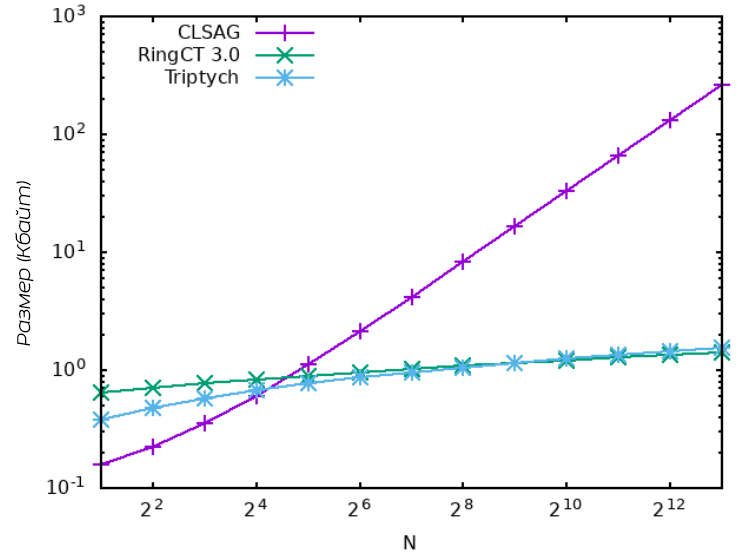
\includegraphics[width=0.6\textwidth]{size.png}
\caption{Размеры доказательств для анонимной группы входа с размером $N$}
\label{fig:size}
\end{figure}


\section{Будущая работа}
Существует возможность дальнейшего расширения системы доказательства Triptych таким образом, чтобы она поддерживала доказательство знания открытий множества обязательств в пределах \textit{одной и той же} анонимной группы и позволяла создавать связующие теги для каждого открытия и демонстрировать баланс напрямую в пределах одного доказательства.
Такая структура, будучи интегрированной в протокол транзакций, будет гораздо эффективнее, чем та, что представлена в настоящей работе, но определения безопасности, применимые к такой структуре, пока ещё проходят оценку.

\bibliographystyle{plain}
\bibliography{main}

\end{document}